\begin{center}
  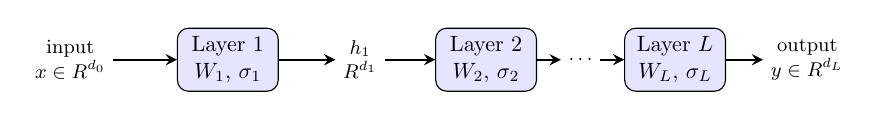
\begin{tikzpicture}[
    scale=0.8, transform shape,
    >=stealth,
    layer/.style={draw, rounded corners, fill=blue!10,
      minimum width=1.6cm, minimum height=1cm, align=center},
    value/.style={align=center, font=\small}
  ]
    \node[value] (x) at (0,0) {input\\\(x \in \mathbb{R}^{d_0}\)};
    \node[layer] (l1) at (2.5,0) {Layer 1\\\(W_1,\,\sigma_1\)};
    \node[value] (h1) at (4.6,0) {\(h_1\)\\\(\mathbb{R}^{d_1}\)};
    \node[layer] (l2) at (6.6,0) {Layer 2\\\(W_2,\,\sigma_2\)};
    \node[value] (dots) at (8.1,0) {\(\cdots\)};
    \node[layer] (lL) at (9.6,0) {Layer \(L\)\\\(W_L,\,\sigma_L\)};
    \node[value] (y) at (11.7,0) {output\\\(y \in \mathbb{R}^{d_L}\)};

    \draw[->, thick] (x) -- (l1);
    \draw[->, thick] (l1) -- (h1);
    \draw[->, thick] (h1) -- (l2);
    \draw[->, thick] (l2) -- (dots);
    \draw[->, thick] (dots) -- (lL);
    \draw[->, thick] (lL) -- (y);
  \end{tikzpicture}

  \medskip
  \(h_0=x,\qquad h_\ell=\sigma_\ell(W_\ell h_{\ell-1}),\qquad y=h_L\)
\end{center}
